%
% File acl2020.tex
%
%% Based on the style files for ACL 2020, which were
%% Based on the style files for ACL 2018, NAACL 2018/19, which were
%% Based on the style files for ACL-2015, with some improvements
%%  taken from the NAACL-2016 style
%% Based on the style files for ACL-2014, which were, in turn,
%% based on ACL-2013, ACL-2012, ACL-2011, ACL-2010, ACL-IJCNLP-2009,
%% EACL-2009, IJCNLP-2008...
%% Based on the style files for EACL 2006 by 
%%e.agirre@ehu.es or Sergi.Balari@uab.es
%% and that of ACL 08 by Joakim Nivre and Noah Smith

\documentclass[11pt,a4paper]{article}
\usepackage[hyperref]{acl2020}
\usepackage{times}
\usepackage{latexsym}
\usepackage{graphicx}

\renewcommand{\UrlFont}{\ttfamily\small}

% This is not strictly necessary, and may be commented out,
% but it will improve the layout of the manuscript,
% and will typically save some space.
\usepackage{microtype}

\aclfinalcopy % Uncomment this line for the final submission
%\def\aclpaperid{***} %  Enter the acl Paper ID here

%\setlength\titlebox{5cm}
% You can expand the titlebox if you need extra space
% to show all the authors. Please do not make the titlebox
% smaller than 5cm (the original size); we will check this
% in the camera-ready version and ask you to change it back.

\newcommand\BibTeX{B\textsc{ib}\TeX}

\title{Transfer Learning for Offensive Language Detection}
\author{Michael Zeng\\
  School of Information\\
  University of California, Berkeley \\
  {\tt zengm71@berkeley.edu} \\\And
  Yekun  Wang\\
  School of Information\\
  University of California, Berkeley \\
  {\tt myekun.wang@berkeley.edu} \\}

 

\date{}

\begin{document}
\maketitle
\begin{abstract}
Offensive language is pervasive on social media platforms and has received lots of attention from both academia as well as big tech. Manually identifying offensive content can be slow, resource intensive, and non-scalable. In this paper, we present a methodology for building an offensive language classifier, adapting the pre-trained contextual embeddings from various transformer models to a text identification architecture, to predict the offensive label for a given text. Oftentimes, organizations face the problem of a scarcity of labeled data, which makes training a deep neural network model difficult. To address this issue, we also experiment with transfer learning techniques which take the model fine-tuned on the Jigsaw Multilingual Toxic Comment Classification dataset and evaluate its performance against the Offensive Language Identification dataset \citep{zampierietal2019}, or OLID . Our best model achieves a 93.27\% AUC score against the private Jigsaw test set and 0.7330 F1 score with zero-shot learning against the OLID dataset. We then discuss the viability of this type of modeling strategy as well as outlining future research direction. 
\end{abstract}

\section{Introduction}
Combining the right to freedom of speech and the protection of online anonymity, the issue of offensive language or language toxicity has become increasingly more pervasive among online communities, penetrating many of the large social media platforms. The widespread use of toxic language is not only harmful for user experience and retention, it is also linked to online harassment and bullying incidents, which could deeply impale the victims mentally. Organizations currently employ various semi-automated content moderation solutions which combine automated offensive language tagging along with human validation to police and to protect their user base. 

Generally speaking, offensive language is defined as anything rude, disrespectful or otherwise likely to make someone leave a discussion. In the past, researchers have studied various neural and non-neural machine learning approaches to identify language toxicity \citep{schmidt-wiegand-2017-survey}. More recently, researches have experimented with deep neural networks models for classifying language toxicity. This paper’s contribution to this area are two-fold: 

\begin{itemize}
  \item We apply various pre-trained state-of-the-art deep neural network models to the task of offensive language identification.
  \item We demonstrate zero-shot and few-shot transfer learning techniques by applying the fine-tuned offensive language classifier to a new dataset and evaluate its general performance. 
\end{itemize}

Recently, transformer-based models \citep{DBLP:journals/corr/VaswaniSPUJGKP17} have been widely used in various areas of NLP research and applications. Depending on model specifications, training this kind of model could require estimating hundreds of millions to billions of parameters. Due to their massive size, many NLP practitioners prefer to build upon a pre-trained transformer model by stacking an extra layer on top, which fine-tunes the existing model for task-specific purposes. This paper aims to evaluate the various transformer-based models, such as BERT-base and BERT-large \citep{DBLP:journals/corr/abs-1810-04805}, XLM \citep{DBLP:journals/corr/abs-1901-07291}, XLM RoBERTa \citep{conneau2019unsupervised}, T5 \citep{raffel2019exploring}; fine-tuning them to detect offensive language on the Jigsaw Multilingual Toxic Comment Classification dataset\footnote{https://www.kaggle.com/c/jigsaw-multilingual-toxic-comment-classification/data}.

Another goal of this study is to demonstrate the effectiveness of sequential transfer learning techniques in resolving the practical issue of labeled data scarcity. The general idea behind transfer learning is to take parameters or knowledge from one trained model and apply it to another \citep{ruder-etal-2019-transfer}. In this study, we experiment with both zero-shot and few-shot learning by applying the offensive language classifier trained on the Jigsaw dataset and evaluate the model's performance against the OffensEval dataset \citep{zampierietal2019}. 

The paper is organized as follows. In section 1, we discuss the existing work related to offensive language identification using various NLP techniques. In section 2, we provide details of the transformer models employed in our experiments. In section 3, we discuss the show results of fine-tuning various transformer models on the Jigsaw dataset. In section 4, we discuss and show results for zero-shot and few-shot learning of applying the fine-tuned toxicity model to the OffensEval dataset. In section 5 and 6, we provide a summary and discuss future research directions.

\subsection{Existing Work}

Earlier research looked into feature-based language models for identifying online bullying and hate speech \citep{6406271} and \citep{huang}. More recently, \citep{zampierietal2019} compiled the OffensEval dataset and applied SVM, CNN, BiLSTM models to predicting the language toxicity label. (Kohli et al., 2017) demonstrated a deep learning approach using word-level and character level RNNs with custom embeddings on the Jigsaw dataset. Additionally, \citep{ruder-etal-2019-transfer} outlined the landscape of various transfer learning techniques pertaining to NLP tasks.  

\subsection{Data}
First part of this study focuses on the Jigsaw Multilingual Toxic Comment Classification dataset, published as a part of a Kaggle competition.\footnote{https://www.kaggle.com/c/jigsaw-multilingual-toxic-comment-classification/data} The data consists of English comments from Wikipedia’s talk page edits as well as an expanded version of the Civil Comments dataset. 

Due to the limit on resources, we constructed our Jigsaw training set by taking the entire 2018 dataset, and combined that with all offensive tweets and down-sampled non-offensive ones from the 2019 dataset. The constructed dataset has close to 500K observations with around 133k being offensive, with a targeted positive rate of 50\%.

Interestingly, Jigsaw’s training dataset is English-only, but the test dataset contains other languages. The organizer intended it this way to validate zero-shot transfer learning of models trained on English and apply them to other languages. We take this idea of transfer learning one step further and focus the second part of the paper on validating zero-shot and few-shot transfer learning on the OffensEval Dataset.

The OffensEval Dataset is provided by the International Workshop on Semantic Evaluation, and 2020 is the second year this task is hosted. This paper focuses on the Offensive Language Identification Dataset (OLID) from the 2019 competition, which contains a collection of 14,200 annotated English tweets. 

\begin{table}
\centering
\begin{tabular}{c|cc}
\textbf{DATASET} & \textbf{Jigsaw}                                                        & \textbf{OLID}                                                              \\ \hline
\textbf{TRAIN}   & \begin{tabular}[c]{@{}c@{}c@{}}485,775\\ 133,610 positive \\English Only\end{tabular} & \begin{tabular}[c]{@{}c@{}c@{}}10,000\\ 1,231 positive \\English Only\end{tabular} \\ \hline
\textbf{DEV}     & \begin{tabular}[c]{@{}c@{}c@{}}8,000\\ 1,230 positive \\ Multi-lingual\end{tabular}     & \begin{tabular}[c]{@{}c@{}c@{}}4,200\\ 1,105 positive\\ English Only\end{tabular}  \\ \hline
\textbf{TEST}    & \begin{tabular}[c]{@{}c@{}c@{}}63,812\\ unknown positive\\ Multi-lingual\end{tabular}  & \begin{tabular}[c]{@{}c@{}c@{}}860\\ 240 positive\\ English Only\end{tabular}   \\ \hline
\end{tabular}
\caption{Dataset Summary}\label{tab:dataset}
\end{table}

To compare our model performance against other participants’ submissions, we used the same evaluation metrics mandated by the competition to train our models -- AUC for the Jigsaw dataset and F1 score for the OffensEval dataset. Table \ref{tab:dataset} gives the detailed breakdown of dataset used for experiments.

\subsection{Infrastructure}
We chose the Kaggle notebook as the working environment to set up our experiments and data analysis, because of two major considerations: firstly, the Jigsaw dataset is hosted on Kaggle as part of the competition, which makes the data import step straightforward; secondly, Kaggle allows 30 hours of TPU v3 or V100 GPU time per person per week, an incredible resource for free access to the state-of-the-art hardware. As a comparison, an V100 instance on IBM costs around \$3.5 depending on the memory and disk; Google Colab Pro offers access to TPU but the availability is not guaranteed. Also, Google Colab Pro offers TPU v2, which only has only 8Gb memory per core, while TPU v3 offers 16Gb memory per core. When experimenting with some of the bigger models, such as XLM RoBERTa large, we could fit 16 observations per core in a batch on TPU v3, while TPU v2 could not fit any after the model is loaded. Comparing TPU vs GPU, we found that TPU offers a significant boost to the training time that’s at least 3-5 times shorter than training on V100 even though the latest V100 could have 32 Gb of RAM. Running some of our experiment notebooks on GPU exceeds the maximum allocated time slot of 3 hours. 

\section{Models}
In this study, we experimented with fine-tuning five transformer models to the language toxicity classification task. In the fine-tuning phase, the model is initialized with the pre-trained parameters and then is fine-tuned on the labelled Jigsaw dataset. All models used in this paper are implemented in HuggingFace \citep{wolf2019huggingfaces}, an open-source library for many state-of-the-art transformer architectures under a unified API. Three suits of models are provided: (i) BERT and BERT large, which were the more truthful implementations of the original BERT model; (ii) multi-language BERT such as XLM and XLM-RoBERTa; (iii) encoder-decoder framework such as T5. 

\subsection{BERT}
BERT, short for Bidirectional Encoder Representations from Transformers, is a bidirectional transformer pre-trained on English language using a combination of masked language modeling (MLM) and next sentence prediction (NSP). We intended to leverage the CLS tokens from the raw model and specify it to the downstream toxicity classification task. We picked the case-sensitive models based on the observation that upper-casing generally imply strong emotions in tweets, which should help with our objective of offensive language detection. We included both BERT-base as well as BERT-large to gauge the improvement in performance against the size of the model. Both model implementations, as published on HuggingFace, had been pre-trained on the BookCorpus and English Wikipedia data.

\subsection{Multi-language BERT}
The work on cross-lingual language models (XLMs) extends the generative pretraining for English language understanding to multiple languages and shows the effectiveness of cross-lingual pretraining. Another variation we picked in our experiment is XLM-RoBERTa model, based on Facebook’s RoBERTa model released in 2019, and trained on 2.5TB of filtered CommonCrawl data. 

\subsection{T5}
Asides from BERT or variations of BERT that build on the encoder part of the transformer architecture, we also experimented with T5, an encoder-decoder model pre-trained on a variety of tasks that had been converted into text-to-text format. The training of T5 differs from the BERT based model: we fed the model with token and labels pairs directly, instead of extracting the CLS tokens and stack softmax layer on top for classification. As detailed in \citep{raffel2019exploring}, the T5 model was pre-trained on 750GB of natural English text, obtained by web crawling.


\section{Jigsaw Performance}
The various pre-trained transformer models were then fine-tuned on the Jigsaw Multilingual Toxic Comment Classification dataset for the language toxicity task. For the Jigsaw dataset, we trained each model on the training set for 3 epochs with 1e-5 learning rate. Since the training set is English only, we then trained each model for 3 additional epochs on the dev set which contains non-English language. 

Traditionally, people add a sigmoid affine layer on top of the CLS tokens to fine tune these transformer models while keeping the transformer weights frozen due to constraints on resources. Gaining access to the TPU units allowed us to experiment with freezing or unfreezing the transformer weights and to evaluate various models more comprehensively both in terms of model performance as well as run time. We report the models' performance on the Jigsaw public and private dataset in Table \ref{tab:jigsaw_performance}, using AUC as the metric to be consistent with the competition. 

% Please add the following required packages to your document preamble:
%\usepackage{multirow}
\begin{table*}[]
\centering
\begin{tabular}{l|lccc}
\multicolumn{1}{l|}{\textbf{MODEL}} &
  \multicolumn{1}{l}{\textbf{\begin{tabular}[l]{@{}l@{}}Freeze\\ Transformer\end{tabular}}} &
  \multicolumn{1}{c}{\textbf{\begin{tabular}[c]{@{}c@{}}Jigsaw Public \\ Score (AUC)\end{tabular}}} &
  \multicolumn{1}{c}{\textbf{\begin{tabular}[c]{@{}c@{}}Jigsaw Private \\ Score (AUC)\end{tabular}}} &
  \multicolumn{1}{c}{\textbf{\begin{tabular}[c]{@{}c@{}}Training \\ Time (s)\end{tabular}}} \\ \hline
\multirow{\textbf{BERT   Base}}       & No  & 0.8037 & 0.8026 & 1,452 \\
                                            & Yes & 0.8044 & 0.8011 & 1,413 \\ \hline
\multirow{\textbf{BERT   Large}}      & No  & 0.8184 & 0.8167 & 3,300 \\
                                            & Yes & 0.8089 & 0.8041 & 3,423 \\ \hline
\multirow{\textbf{XLM}}               & No  & 0.9148 & 0.9121 & 2,859 \\
                                            & Yes & 0.9096 & 0.9094 & 2,901 \\ \hline
\multirow{\textbf{XLM Roberta Large}} & No  & \textbf{0.9335} & \textbf{0.9327} & 5,205 \\
                                            & Yes & 0.9306 & 0.9315 & 5,115 \\ \hline
\multirow{\textbf{T5 Large}}          & No  & 0.8392 & 0.8373 & 8,844 \\
                                            & Yes & 0.8371 & 0.8352 & 8,925 \\ \hline
\end{tabular}
\caption{Performance on Jigsaw Dataset and Training Time for 3 Epochs}\label{tab:jigsaw_performance}
\end{table*}

We see an intuitive improvement in performance from unfreezing the transformer weights. By unfreezing the transformer weights, we are allowing many more degrees of freedom while training the model. Yet we see the increase in model power generalizes very well on the test set. On the other hand, unfreezing the transformer weights consumes more memory on the TPU unit, and thus allows lower batch sizes. Yet from our experiment, the training time stayed largely the same, which prompts us to leave the transformer weights unfrozen for the rest of the experiments. 

Comparing across models, the gain from BERT to BERT large is only marginal despite the significant size-up and increase in training time. The big leap in performance came from the switching from English to multi-language models such as XLM and XLM RoBERTa large. Given the fact that both the public and private test sets are multilingual, the English only embedding we used in BERT Base, BERT Large as well as T5 large is limiting the model performance. The improvement from XLM to XLM RoBERTa large could be mostly attributed to the pretraining of XLM Roberta Large, where the model was exposed to and trained on significantly larger corpus. 

\section{Transfer Learning}
% The focus of this paper is to demonstrate the application and extensibility of the Transformer architecture to the text classification problem. Real-world NLP applications are oftentimes limited by the amount of data and computational resources to properly train a deep neural net NLP model. Instead of starting from scratch, a more preferred strategy is to take a model pre-trained on a large body of text and fine-tune it for a specific NLP task. Effectively, it is a type of transfer learning based on the assumption of a commonality in basic language understanding between the pre-trained dataset and the target task dataset. 

In this section, we started by exploring the differences in zero-shot transfer learning performances from multiple models on the OLID dataset. It serves as a reasonable baseline for the model’s ability to generalize to unseen data, given that the model was previously fine-tuned on a very related task. We then explored the performances in few-shot learning by incrementally increase the portion of the OLID data for the model to be trained on. Given that we have 10K in total from the OLID training set, the choice of exposure was set to follow the geometric sequence: 1K, 2K, 5K and 10K. For training, we lowered the learning rate to 2.00E-06 and trained up to 10 epochs with a tight early-stop that checks the loss on dev set every 3 epochs. The hypothesis is that since the model has been pretrained on similar tasks, one would only need to expose a fraction of the dataset to obtain a high level of performance.

\begin{table*}[h]
\centering
\begin{tabular}{l|lccccc}
\textbf{Model}                              & \textbf{Freeze} & \textbf{OLID 0-shot} & \textbf{OLID 1k} & \textbf{OLID 2k} & \textbf{OLID 5k} & \textbf{OLID 10k (Full)} \\ \hline
\multirow{\textbf{BERT Base}}  & No  & 0.6690 & 0.6847 & 0.6821 & 0.6944 & 0.7091 \\
                               & Yes & 0.6226 & 0.6283 & 0.6283 & 0.6455 & 0.6750  \\ \hline
\multirow{\textbf{BERT Large}} & No  & 0.6919 & \textbf{0.7018} & \textbf{0.7065} & \textbf{0.7253} & \textbf{0.7330} \\
                               & Yes & 0.6619 & 0.6595 & 0.6596 & 0.6619 & 0.6690 \\ \hline
\multirow{\textbf{XLM}}        & No  & 0.6502 & 0.6655 & 0.6786 & 0.6969 & 0.7055 \\
                               & Yes & 0.6283 & 0.6285 & 0.6490 & 0.6513 & 0.6537 \\ \hline
\multirow{\textbf{XLM Roberta Large}} & No              & 0.6631               & 0.6762           & 0.7029           & 0.7091           & 0.7104            \\
                               & Yes & \textbf{0.6942} & 0.6895 & 0.6980 & 0.7029 & 0.7042 \\ \hline
\multirow{\textbf{T5}}         & No  & 0.6675 & 0.6838 & 0.6994 & 0.7072 & 0.7091 \\
                               & Yes & 0.6664 & 0.6663 & 0.6667 & 0.6669 & 0.6683 \\ \hline
\end{tabular}
\caption{Performance of Transfer Learning on OLID Dataset}\label{tab:olid_performance}
\end{table*}

\begin{figure}[h]
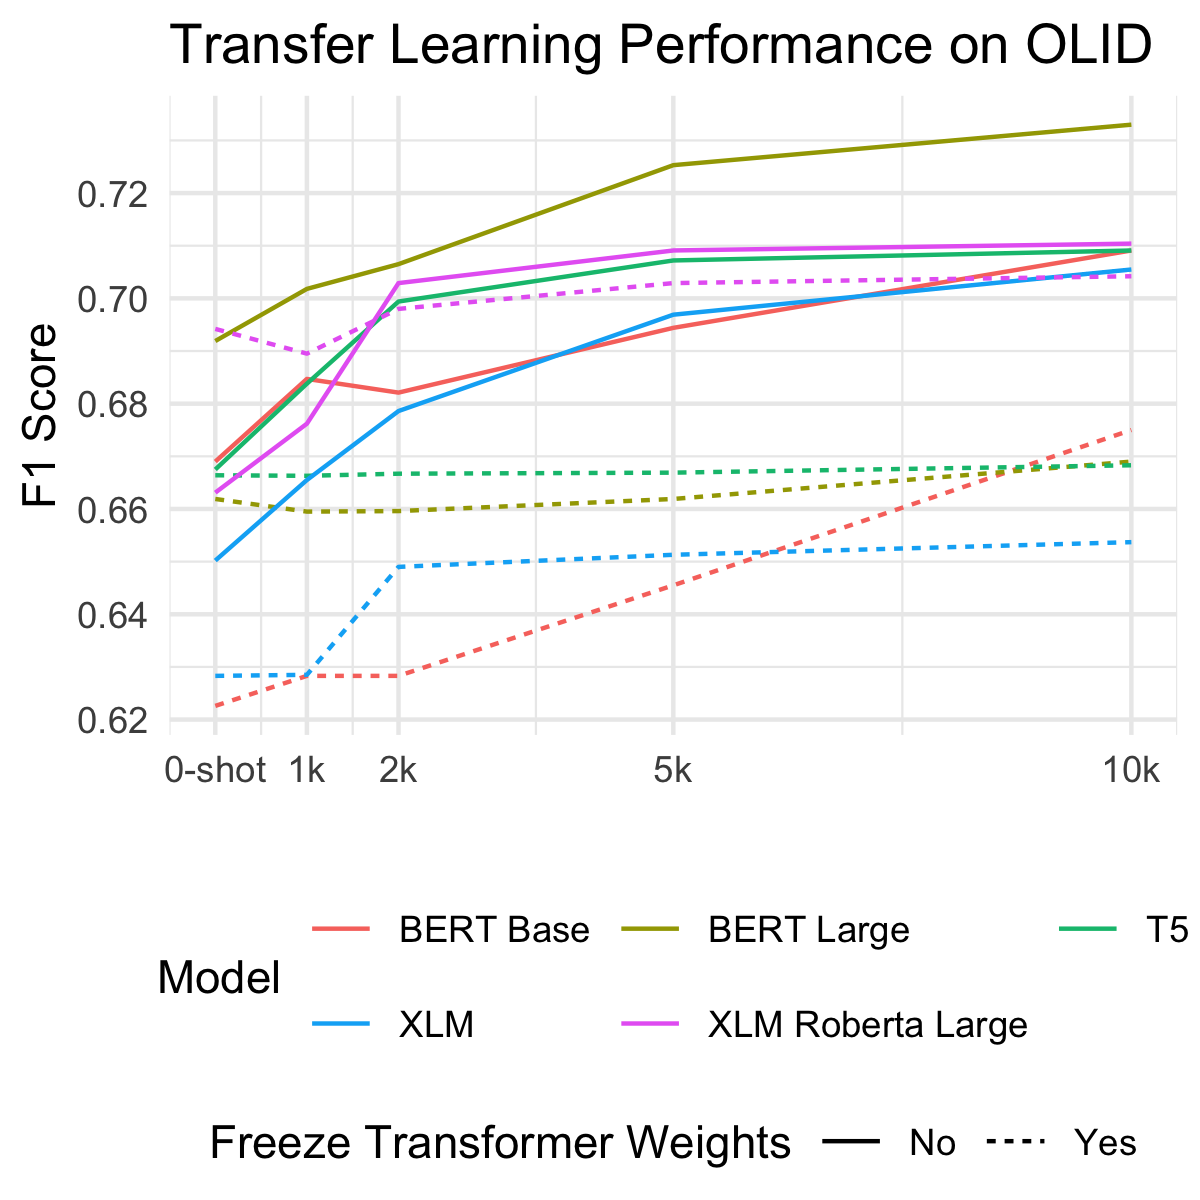
\includegraphics[width=\columnwidth]{transfer_learning_performance_nominal.png}
\centering
\caption{Performance of Transfer Learning on OLID Dataset}\label{fig:olid_performance_fig}
\end{figure}

Table \ref{tab:olid_performance} summarises the F1 score on the OLID test set from various experiments, which are further visualized in Figure \ref{fig:olid_performance_fig}. Our observations on the choice of freezing the transformer weights from the previous section still hold: most models perform better when trained with weights from transformer layer unfrozen. When they are frozen, the performance curves stayed mostly flat as more destination dataset is exposed. This indicates a lack of flexibility to adapt and learn from the new dataset with only the last layer being trainable.  

Across the different models, we found that BERT-large consistently outperforms the others across the zero-shot and few-shot experiments. We no longer observe performances leaps from multi-lingual model such as XLM and XLM RoBERTa Large since the OLID test set is English only. 

As more observations are exposed to the model, we observe the performances continue to improve but at diminshing rates, as shown in Figure \ref{fig:olid_performance_fig}. For most models trained with weights from the transformation layer unfrozen, exposing the entire training set helps achieve about a 4\% gain in F1 score compared to doing zero-shot inference, yet most of the gain was achieved from the first 5k observations. This is similar to the findings in \citep{cer2018universal}, where the author demonstrated that the performances would plateau as more labeled examples are exposed to the model. However, we are still trying to procure more labeled data on offensive language detection so that we can expand our experiment beyond 10k observations to observe the curve over large ranges.  

\section{Conclusion}
We explored the both zero and few-shots learning performances across several popular transformer based models within the common task of offensive language detection. Our experiments show unfreezing the weights from transformer layer, if resources allow, greatly boosts the model's ability to generalize and perform on unseen dataset. In terms of few-shots learning, we observed diminishing returns from exposing the model to additional training examples, as first cited in \citep{cer2018universal}. However, the performance of zero or few-shots learning are also largely limited by the language in which the model was originally pretrained on: XLM RoBERTa has superior performance on Jigsaw test set which is multi-lingual, while BERT performs the best on OLID test set which is English only. 

\bibliography{acl2020}
\bibliographystyle{acl_natbib}
\end{document}
